% Neural network diagram
% Made with Xematics. Positions are in px (1 px = 0.75 pt), as in the SVG export.
\documentclass[tikz, border=4pt]{standalone}
\usepackage{amsmath, amssymb}
\definecolor{xm1}{HTML}{FFFFFF}
\definecolor{xm2}{HTML}{D9D9D9}
\definecolor{xm3}{HTML}{000000}
\definecolor{xm4}{HTML}{595959}
\definecolor{xm5}{HTML}{A6A6A6}
\definecolor{xm6}{HTML}{4D4D4D}
\begin{document}
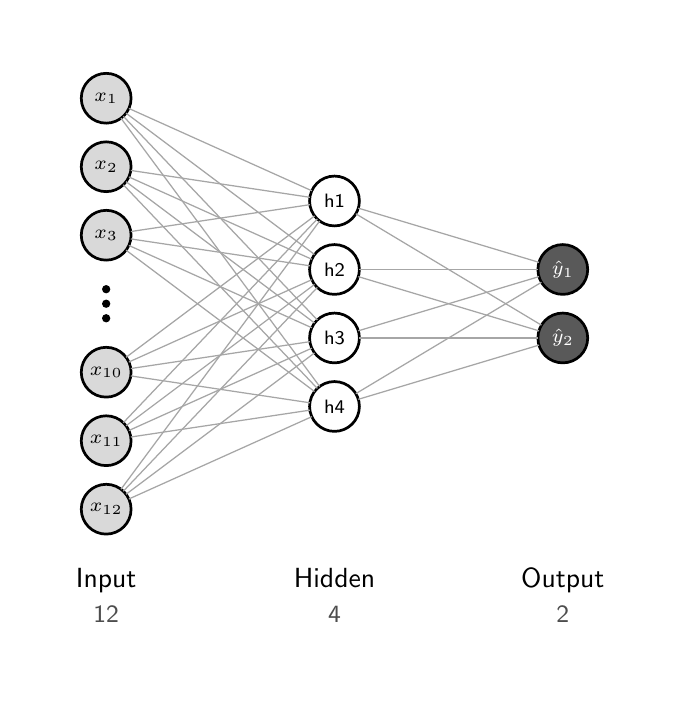
\begin{tikzpicture}[x=0.75pt, y=-0.75pt]
  \tikzset{
    xm input/.style={circle, minimum size=18pt, inner sep=0, outer sep=0, fill=xm2, draw=xm3, line width=0.98pt},
    xm hidden/.style={circle, minimum size=18pt, inner sep=0, outer sep=0, fill=xm1, draw=xm3, line width=0.98pt},
    xm output/.style={circle, minimum size=18pt, inner sep=0, outer sep=0, fill=xm4, draw=xm3, line width=0.98pt},
    xm edge/.style={draw=xm5, line width=0.45pt},
    xm dots/.style={fill=xm3},
    xm nodelabel xm3/.style={text=xm3, inner sep=0, font=\sffamily\fontsize{7.5}{9}\selectfont},
    xm nodelabel xm1/.style={text=xm1, inner sep=0, font=\sffamily\fontsize{7.5}{9}\selectfont},
    xm name xm3/.style={text=xm3, inner sep=0, font=\sffamily\fontsize{9.75}{11.7}\selectfont},
    xm size xm6/.style={text=xm6, inner sep=0, font=\sffamily\fontsize{9}{10.8}\selectfont},
  }
  \fill[xm1] (0,0) rectangle (301.07,311.25);
  % Neurons
  \node[xm input] (n-0-0) at (37.82,34) {};
  \node[xm input] (n-0-1) at (37.82,67) {};
  \node[xm input] (n-0-2) at (37.82,100) {};
  \node[xm input] (n-0-9) at (37.82,166) {};
  \node[xm input] (n-0-10) at (37.82,199) {};
  \node[xm input] (n-0-11) at (37.82,232) {};
  \node[xm hidden] (n-1-0) at (147.82,83.5) {};
  \node[xm hidden] (n-1-1) at (147.82,116.5) {};
  \node[xm hidden] (n-1-2) at (147.82,149.5) {};
  \node[xm hidden] (n-1-3) at (147.82,182.5) {};
  \node[xm output] (n-2-0) at (257.82,116.5) {};
  \node[xm output] (n-2-1) at (257.82,149.5) {};
  % Connections 0
  \draw[xm edge] (n-0-0) -- (n-1-0);
  \draw[xm edge] (n-0-0) -- (n-1-1);
  \draw[xm edge] (n-0-0) -- (n-1-2);
  \draw[xm edge] (n-0-0) -- (n-1-3);
  \draw[xm edge] (n-0-1) -- (n-1-0);
  \draw[xm edge] (n-0-1) -- (n-1-1);
  \draw[xm edge] (n-0-1) -- (n-1-2);
  \draw[xm edge] (n-0-1) -- (n-1-3);
  \draw[xm edge] (n-0-2) -- (n-1-0);
  \draw[xm edge] (n-0-2) -- (n-1-1);
  \draw[xm edge] (n-0-2) -- (n-1-2);
  \draw[xm edge] (n-0-2) -- (n-1-3);
  \draw[xm edge] (n-0-9) -- (n-1-0);
  \draw[xm edge] (n-0-9) -- (n-1-1);
  \draw[xm edge] (n-0-9) -- (n-1-2);
  \draw[xm edge] (n-0-9) -- (n-1-3);
  \draw[xm edge] (n-0-10) -- (n-1-0);
  \draw[xm edge] (n-0-10) -- (n-1-1);
  \draw[xm edge] (n-0-10) -- (n-1-2);
  \draw[xm edge] (n-0-10) -- (n-1-3);
  \draw[xm edge] (n-0-11) -- (n-1-0);
  \draw[xm edge] (n-0-11) -- (n-1-1);
  \draw[xm edge] (n-0-11) -- (n-1-2);
  \draw[xm edge] (n-0-11) -- (n-1-3);
  % Connections 1
  \draw[xm edge] (n-1-0) -- (n-2-0);
  \draw[xm edge] (n-1-0) -- (n-2-1);
  \draw[xm edge] (n-1-1) -- (n-2-0);
  \draw[xm edge] (n-1-1) -- (n-2-1);
  \draw[xm edge] (n-1-2) -- (n-2-0);
  \draw[xm edge] (n-1-2) -- (n-2-1);
  \draw[xm edge] (n-1-3) -- (n-2-0);
  \draw[xm edge] (n-1-3) -- (n-2-1);
  % Layers
  \fill[xm dots] (37.82,126) circle[radius=2];
  \fill[xm dots] (37.82,133) circle[radius=2];
  \fill[xm dots] (37.82,140) circle[radius=2];
  % Labels
  \node[xm nodelabel xm3, anchor=center] at (37.82,34) {$x_{1}$};
  \node[xm nodelabel xm3, anchor=center] at (37.82,67) {$x_{2}$};
  \node[xm nodelabel xm3, anchor=center] at (37.82,100) {$x_{3}$};
  \node[xm nodelabel xm3, anchor=center] at (37.82,166) {$x_{10}$};
  \node[xm nodelabel xm3, anchor=center] at (37.82,199) {$x_{11}$};
  \node[xm nodelabel xm3, anchor=center] at (37.82,232) {$x_{12}$};
  \node[xm nodelabel xm3, anchor=center] at (147.82,83.5) {h1};
  \node[xm nodelabel xm3, anchor=center] at (147.82,116.5) {h2};
  \node[xm nodelabel xm3, anchor=center] at (147.82,149.5) {h3};
  \node[xm nodelabel xm3, anchor=center] at (147.82,182.5) {h4};
  \node[xm nodelabel xm1, anchor=center] at (257.82,116.5) {$\hat{y}_{1}$};
  \node[xm nodelabel xm1, anchor=center] at (257.82,149.5) {$\hat{y}_{2}$};
  \node[xm name xm3, anchor=base] at (37.82,269.59) {Input};
  \node[xm size xm6, anchor=base] at (37.82,286.35) {12};
  \node[xm name xm3, anchor=base] at (147.82,269.59) {Hidden};
  \node[xm size xm6, anchor=base] at (147.82,286.35) {4};
  \node[xm name xm3, anchor=base] at (257.82,269.59) {Output};
  \node[xm size xm6, anchor=base] at (257.82,286.35) {2};
\end{tikzpicture}
\end{document}
